
\chapter{Experimental evaluation: the service coverage problem \label{chap:Experimental-evaluation-the-service-coverage-problem}}

% First paragraph has no indentation.

In the context of coverage planning and control, the power of the
CPICH signal determines the coverage area of the cell. It also impacts
the network capacity, and thus the quality of service. Pilot power
is the parameter that allows us to control the strength of the CPICH
signal. A higher power for pilot signals means better coverage. On
the other hand, more pilot power translates in decreased network capacity.

We consider the problem of minimizing the total amount of pilot power
subject to a full coverage constraint. Our optimization approach,
based on parallel autonomous agents, gives very good solutions to
the problem within an acceptable amount of time. The parallel implementation
takes full advantage of GPU hardware in order to achieve impressive
speed-up. We report the results of our experiments for three UMTS
networks of different sizes based on a real network currently deployed
in Slovenia.


\section{Introduction}

The coverage problem in third-generation (3G) mobile networks has
received a great deal of attention in the last years. Its complexity
demands the confluence of different skills in areas such as propagation
of radio signals, telecommunications and information systems, among
others.

The problem becomes even more complex as conflicting measures to compare
different proposed solutions are taken into account. These aspects
include network capacity, quality of service, service coverage, and,
recently, issues related with human exposure to electromagnetic fields
generated by base station antennas \cite{Esposito_Genetic.optimization.for.optimum.3G.network.planning:2010}.
Public opinion has been extremely sensitive regarding this issue,
and thus many countries have already imposed safety standards to limit
the electromagnetic field levels.

It is clear that even after almost 10 years after the launch of the
first commercial UMTS network, service coverage planning remains a
key problem that all mobile operators have to deal with. Its intricacy
arises from the wide range of different combinations of configuration
parameters and their evaluation-time complexity. One crucial parameter,
which is mainly subject of adjustment, is the transmit power of the
common pilot channel (CPICH). The CPICH transmit power is common to
many different planning and optimization problems in UMTS networks
\cite{Nawrocki_Understanding:2006}.

The CPICH transmits in the downlink of a UMTS cell system. The transmit
power is usually between 5\% and 10\% of the total power available
at the base station \cite{Holma_WCDMA.for.UMTS:2005}. The capacity
of a cell is limited by the amount of available power at the base
station and the interference level at the mobile terminal. The coverage
area of any cell is controlled by changing its pilot power, which
consequently modifies the service area of the network.

From the network perspective, minimizing pilot power usage leaves
more power available for increased network capacity. This is especially
important if the traffic and other channels are configured relative
to CPICH \cite{Holma_WCDMA.for.UMTS:2005}. Moreover, as applications
demand for mobile internet access and data services increases \cite{Cunningham_Network.growth.theory.and.evidence:2010},
so does the pressure on existing network infrastructure, making parameter
optimization the only viable short-term solution \cite{Nawrocki_Understanding:2006}.

There are different approaches in the literature that are able to
solve the coverage problem \cite{Nawrocki_Understanding:2006,Siomina_Pilot.power.optimization:2004}.
Some of them even claim to achieve near-optimal solutions \cite{Siomina:Minimum.pilot.power.for.service.coverage}.
As a matter of fact, such formulations have proven useful only for
small network instances and often fail when challenged with real-world
networks.

The idea of using autonomous agents for optimization is not new. It
has proven to be a solid optimization approach for solving different
types of problems, not only within the area of mobile networks \cite{Esposito_Genetic.optimization.for.optimum.3G.network.planning:2010,Cheung_Realtime.video.using.agent.over.3G.networks:2005},
but also in other fields \cite{Vasile_Hybrid.multiagent.approach.for.optimization:2009,Valcarce_Applying.FDTD.to.the.coverage.prediction.of.WiMAX:2009}.
Nevertheless, we have not observed any similar optimization method
for solving the service coverage problem in mobile networks \cite{Benedicic_Pilot.power.optimization:2010}.
Moreover, this is, to the best of our knowledge, the first work to
experiment with optimization of a real UMTS network on a fully-enabled
GPU environment.

Our optimization approach is based on a state-of-the-art mathematical
model, that has been previously used to solve a comparable problem
\cite{Chen-Yuan_CPICH.optimization:2008}. We tackle the problem of
computational-time complexity when dealing with big problem instances
by implementing a parallel version of our agent-based algorithm entirely
on GPU. This minimizes overhead when deploying a larger number of
agents working in parallel over the service area, limited only by
the amount of memory available. 

We tested our algorithm on subsets of a real UMTS network deployed
in Slovenia. All network-related data were provided by the mobile
operator Mobitel Telecommunication Services, Inc. The results show
that the solutions found, and more importantly their quality, are
greatly improved when compared to other common planning techniques.

We begin our discussion by introducing previous work and a description
of the coverage problem, where we formally introduce some of its key
elements. We then discuss our parallel-agent approach in detail, as
well as the strategies used for result comparison. Having introduced
the parallel-agent approach, we move on to describe the GPU implementations
of its two key elements: the objective-function evaluator and the
agents. Simulations and experimentation, performed on three sub-networks
of a real mobile network deployed in Slovenia, follow. We conclude
with an overview of the achieved results, from the optimization as
well as the implementation points of view, and discuss future research
directions.


\section{Previous work}

In \cite{Siomina:Minimum.pilot.power.for.service.coverage}, Siomina
and Yuan considered the problem of minimizing the total amount of
pilot power subject to a full coverage constraint. They tackled the
problem with an iterative linear programming approach, reporting very
good results for some small-sized test networks. The authors also
noted that bigger problem instances could not be solved because of
hardware constraints on the target platform.

In a different work \cite{Benedicic_Pilot.power.optimization:2010},
we tackled the full-coverage problem of the service area under optimization.
Reported experimentation on the same problem instances as in \cite{Siomina:Minimum.pilot.power.for.service.coverage}
showed improved quality at the cost of longer running time. Moreover,
our approach was not limited by any hardware restrictions, since it
successfully tackled bigger problem instances, finding high quality
solutions even for large networks. Such solutions were found in a
reduced amount of time by increasing the number of agents deployed
during optimization without compromising solution quality.

The algorithm in \cite{Benedicic_Pilot.power.optimization:2010} is
the basis for the optimization algorithm presented in this paper,
with some essential improvements, namely:
\begin{itemize}
\item the original implementation was completely CPU-based and used a black-box
coverage evaluator;
\item the algorithm presented here contains improvements in the agent's
behavior during optimization, including the introduction of the so-called
``special'' agents and some fine-tuning of their step sets.
\end{itemize}

\section{Problem description}

In the problem of optimization of pilot powers for service coverage,
the objective is to find a set of pilot power settings for all cells
in the network, such that the total pilot power used is minimized,
and a given service coverage criteria is fulfilled. We consider the
pilot power minimization problem subject to a full coverage constraint
of the service area.

Because the mathematical model of the problem is not of primary interest
here, we will just outline it, so that all problem elements are formally
defined and represented. For additional information regarding mathematical
models of comparable problems, see \cite{Nawrocki_Understanding:2006}.


\subsection{Problem elements}

We start by considering a UMTS network of $m$ cells and use $C$
to denote the set of cells, i.e. $C=\{1,...,m\}$. A pixel grid of
a given resolution represents the service area for which the signal
propagation predictions are known. Let $n$ denote the total number
of pixels in the service area and let $S$ denote the pixel set, i.e.
$S=\{1,...,n\}$. We also denote $att_{cs}$, $0\le att_{cs}\le1$,
as the attenuation factor between a cell $c$ and a pixel $s$, which
is calculated by performing signal propagation predictions for every
pair of $c\in C$ and $s\in S$.

For every $c\in C$, we define $p_{c}^{T}$ as the total transmission
power available in cell $c$. This power is shared among all channels
in the cell (i.e. CPICH, other common channels, and dedicated traffic
channels). We define $p_{c}$ as the amount of power allocated to
the pilot signal of cell $c$, where $p_{c}$ may adopt any value
from a finite set of possible pilot power levels, $P_{c}=\{p_{c}^{1},p_{c}^{2},...,p_{c}^{T}\}$.
Consequently, the received pilot power of cell $c$ in pixel $s$
is $att_{cs}p_{c}$.

Considering the full coverage constraint, each pixel in the service
area should have at least one cell covering it. We assume that a pixel
$s$ is under coverage of a cell $c$ if its signal-to-interference
ratio, $SIR$, at pixel $s$ is not lower than a given threshold,
$\gamma_{c}$, i.e.

\begin{equation}
SIR(c,s)=\frac{p_{c}att_{cs}}{\sum_{i\in C}p_{i}^{T}att_{is}+\tau_{0}}\ge\gamma_{c}\label{eq:sir}
\end{equation}


where $\tau_{0}$ is the thermal noise. In (\ref{eq:sir}), we are
assuming that all cells in the network operate at full power, which
is the worst case scenario. This ensures that even under heavy user
traffic, full coverage of the service area is maintained, because
of the cell-breathing principle \cite{Holma_WCDMA.for.UMTS:2005}.
The same assumption has also been used in \cite{Siomina:Minimum.pilot.power.for.service.coverage,Chen-Yuan_CPICH.optimization:2008}.

The optimization problem corresponds to finding the pilot power levels
$p_{c}$, for all cells $c\in C$, such that coverage of at least
$b$ pixels is guaranteed, while the total amount of pilot power used
is minimized. Since we are considering full coverage, we denote $b=n$.


\subsection{Problem complexity \label{sub:Problem-complexity}}

It has been proved that the problem of pilot power optimization for
full coverage of the service area is $NP$-hard, since it can be reduced
to the set covering problem \cite{Varbrand_Mathematical.programming.approach:2003}.
Consequently, as long as $P\neq NP$, it is unfeasible that a polynomial-time
algorithm exists, which is able to find an exact solution to this
problem.


\subsection{Optimization objective and constraints}

The optimization objective is defined as follows

\begin{equation}
P^{*}=\min\sum_{c\in C}p_{c};\label{eq:objective_function-1}
\end{equation}


subject to

\begin{equation}
\frac{\sum_{s\in S}cov(s)}{b}=1,\label{eq:coverage_constraint}
\end{equation}


where

\begin{equation}
cov(s)=1\,\,\, if\, and\, only\, if\,\,\,\exists c\vert SIR(c,s)\ge\gamma_{c}\label{eq:coverage}
\end{equation}


\[
cov(s)=0\,\,\, otherwise
\]


The definition of (\ref{eq:coverage}) provides us a simple way of
asserting the coverage of a given pixel, $s$. It follows that if
the pilot signal of at least one cell $c$ satisfies the imposed $SIR$
threshold, $\gamma_{c}$, the pixel is covered and hence $cov(s)=1$.


\section{Optimization approaches \label{sec:Solution-approaches}}

Since the problem instances we will be analyzing are part of a real
mobile network deployed in Slovenia by Mobitel Telecommunication Services,
Inc., there are no references in the literature of other optimization
techniques dealing with exactly the same data set. For this reason,
we will introduce two different strategies for setting the pilot power,
that shall enable us to compare the experimentation results. The first
strategy is attenuation-based pilot power, presented in \cite{Siomina_Pilot.power.optimization:2004},
in which a pixel of the service area is always covered by the cell
with the highest attenuation-factor value. The second strategy is
our parallel-agent approach, based on ideas inspired by two-dimensional
cellular automata \cite{Sarkar_Cellular.automata.history:2000} and
metaheuristics \cite{Talbi_Metaheuristics:2009}. A detailed description
is given in section \ref{sub:Parallel-multi-agent-approach}.

Similar criteria for result comparison have also been used in \cite{Siomina:Minimum.pilot.power.for.service.coverage}.


\subsection{Attenuation-based pilot power}

The first heuristic for setting the pilot power of all cells in the
network is known as attenuation-based, since it relies on the attenuation
factor, $att_{cs}$. A pixel of the service area, $s$, is always
covered by the cell exhibiting the maximum $att_{cs}$. Whenever the
maximum available power, $p_{c}^{T}$, is the same for all the cells
in the network, this is equivalent to selecting the cell with the
minimum required pilot power to cover pixel $s$. Hence, under this
assumption, we identify the cell $c$ covering pixel $s$ as

\begin{equation}
p_{c(s)}=\min_{c\in C}p_{cs}\label{eq:attenuation_based-power}
\end{equation}


Picking the cells conforming to (\ref{eq:attenuation_based-power})
and setting the pilot powers accordingly, we achieve full coverage
of the service area with a solution exhibiting a total pilot power
of

\begin{equation}
P^{Att}=\sum_{c\in C}\max p_{c(s)}
\end{equation}


The procedure to find a cell $c(s)$ for every pixel in the service
area consists in sorting, in descending order, all pixels by the maximum
attenuation factor value, $att_{cs}$, among all cells, i.e. $att_{c(s),s}$.
The solution is thus established by the first $b$ pixels of the sorted
sequence, taking the maximum pilot power setting for a cell into account,
i.e. $p_{c(s)}$.


\subsection{Parallel-agent approach \label{sub:Parallel-multi-agent-approach}}

In the parallel-agent approach, a set of autonomous worker agents
explore the geographic area, targeted to be under mobile network coverage,
in order to optimize the pilot power consumption of the network. Each
agent randomly moves over the service area as it dictates different
changes to the pilot power of the cells. An objective-function evaluator
performs radio propagation predictions based on each agent's proposed
change.

The search process during optimization is strictly random. However,
several physical properties that are exclusive to the problem being
solved are being exploited during exploration of the search space.
Additionally, whenever the current solution breaks any of the given
constraints, the optimization process is guided back to the space
of valid solutions, providing a mechanism for improving exploration
and escaping from local optima.

Because of the independent nature in agent's behavior, a parallel
implementation is fairly straightforward to achieve. The first hardware
restriction we have to overcome is the amount of memory on the GPU
device. Consequently, careful memory utilization and organization
are critical to successfully accommodate all involved problem elements
on the GPU. Figure \ref{fig:Architecture} gives an overview of the
optimization system architecture. Within this GPU-only architecture,
agents work in a parallel and autonomous manner, while the evaluator
reacts to agents' changes.

\begin{figure}
\centering

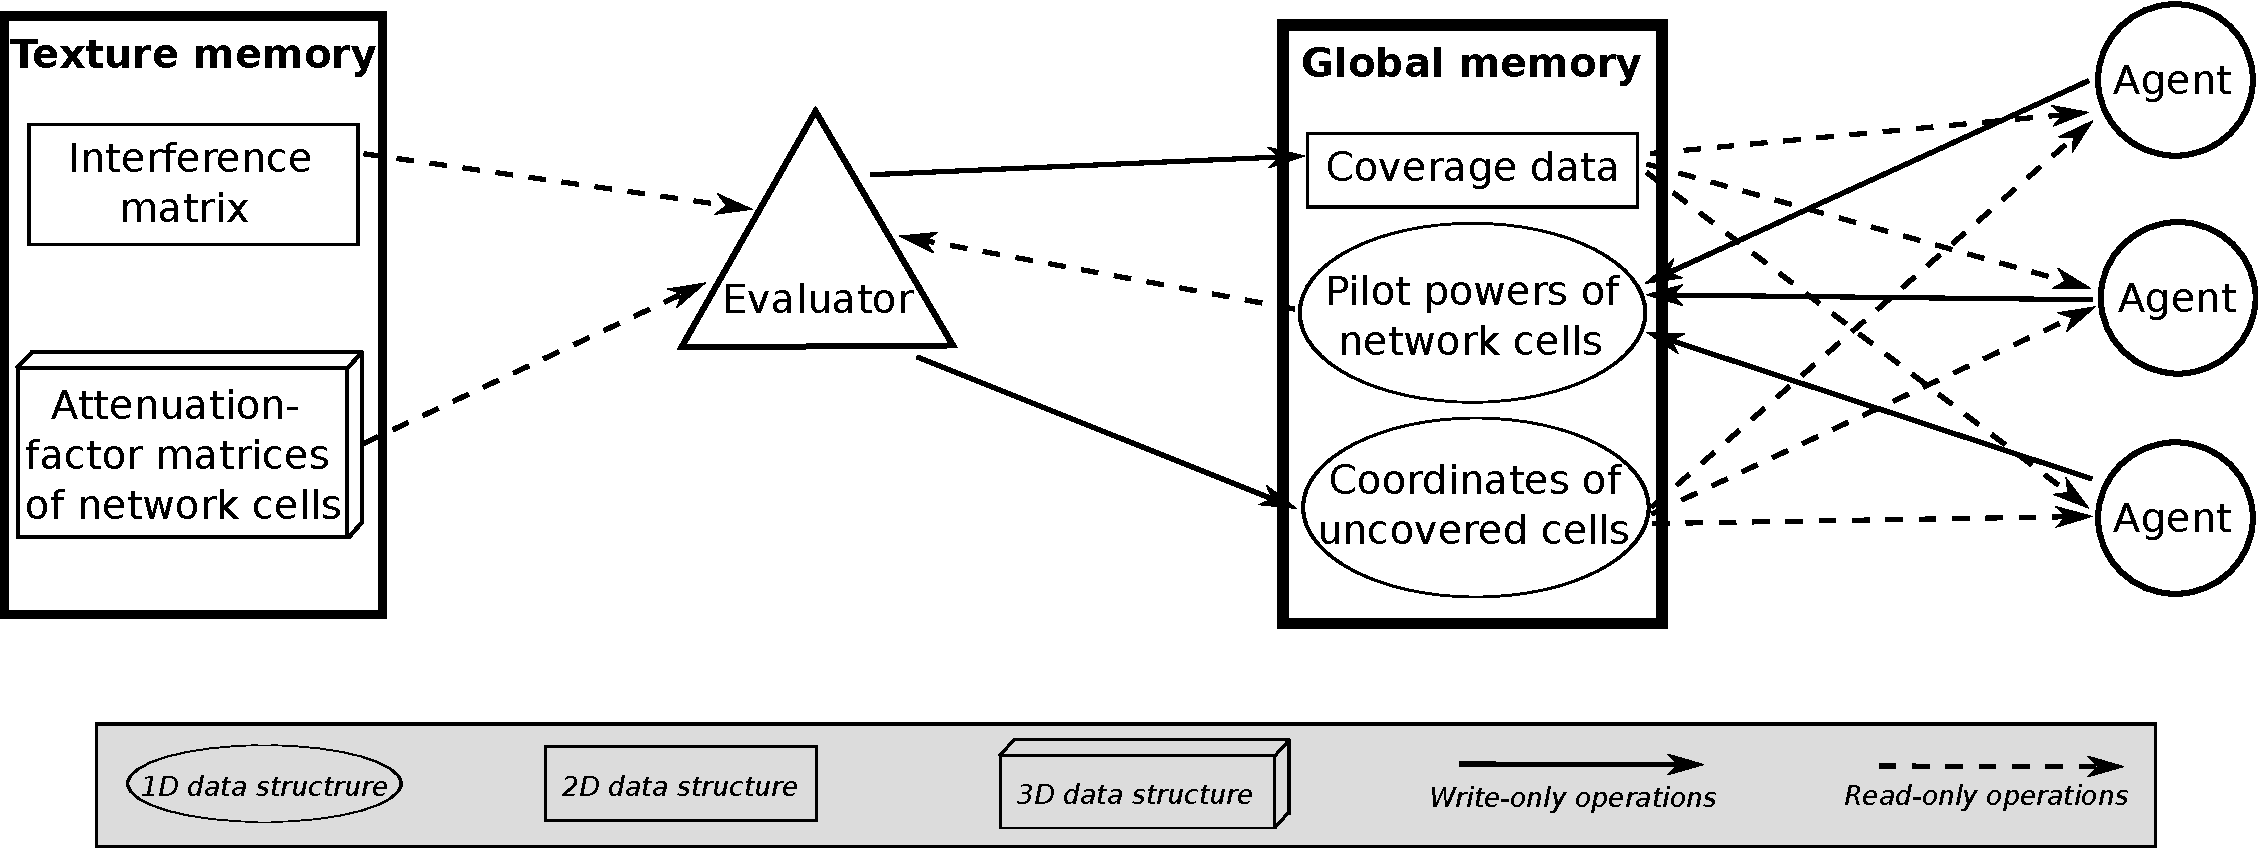
\includegraphics[width=1\textwidth]{06-experimental_evaluation-service_coverage/img/architecture}

\caption{\textit{Architecture of the optimization system on GPU.\label{fig:Architecture}}}
\end{figure}



\subsubsection{The agents}

The agents apply the pilot power changes based exclusively on local
information. Each of them encapsulates a set of steps that is consistently
applied as it randomly moves through the service area of the network.
Whenever an agent arrives at a pixel $s$, it identifies the set of
cells covering the current pixel, namely 

\begin{equation}
B(s)=\{c\in C\mid SIR(c,s)\ge\gamma_{c}\}
\end{equation}


\begin{table}
\caption{\textit{Pseudo-code of the agent's behavior.\label{tab:Agent-behavior}}}


\centering

\begin{tabular}{c|l}
\hline 
Step & \tabularnewline[\doublerulesep]
\hline 
 & $\mathbf{repeat}$\tabularnewline
1 & $\,\,\,\,\mathbf{if}\, Special\, agent\,(\,)\,\mathbf{and}\,|U|>0\,\mathbf{then}$\tabularnewline
2 & $\,\,\,\,\,\,\,\, s=random\, element\, from\, U$\tabularnewline
 & $\,\,\,\,\mathbf{else}$\tabularnewline
3 & $\,\,\,\,\,\,\,\, s=random\, element\, from\, S$\tabularnewline
 & $\,\,\,\,\mathbf{end\, if}$\tabularnewline
4 & $\,\,\,\, move\, to\, s$\tabularnewline
5 & $\,\,\,\,\mathbf{if}\,|B(s)|=0\,\mathbf{then}$\tabularnewline
6 & $\,\,\,\,\,\,\,\, apply\, SS_{0}\,\,\,\,//increase\, power$\tabularnewline
7 & $\,\,\,\,\mathbf{else\,}\mathbf{if}\,|B(s)|\ge1\,\mathbf{then}$\tabularnewline
8 & $\,\,\,\,\,\,\,\, apply\, SS_{1}\,\,\,\,//decrease\, power$\tabularnewline
 & $\,\,\,\,\mathbf{end\, if}$\tabularnewline
 & $\mathbf{while\,}\mathbf{not}\,(stopping\, criteria)$\tabularnewline
\hline 
\end{tabular}
\end{table}


The step set applied from this point on directly depends on the cardinality
of $B(s)$, while the agent's movement over the service area is determined
by the cardinality of set $U$, $U\subset S$, which is defined as

\begin{equation}
U=\{s\in S\mid\forall c\in C:SIR(c,s)<\gamma_{c}\}
\end{equation}


The agent's behavior is dictated by the pseudo-code shown in Table
\ref{tab:Agent-behavior}. Steps 1 to 4 are responsible for guiding
the agent's movement. The coordinates are selected randomly from two
sets. The first, $S$, is the set of all pixels in the service area.
The other one, $U$, is the set of pixels that are currently not being
covered by the network. Only ``special'' agents may select pixel
coordinates of the set $U$. It follows, that an agent's movement
depends on its ``specialty'' and the number of pixels not covered
by the current solution. During steps 5 to 8, the agent applies step
sets $SS_{0}$ and $SS_{1}$ based on the number of cells in $B(s)$.

\begin{table}
\caption{\textit{Pseudo-code of step set $SS_{0}$.\label{tab:Rule-set-0}}}


\centering

\begin{tabular}{c|l}
\hline 
Step & \tabularnewline[\doublerulesep]
\hline 
 & $\mathbf{repeat}$\tabularnewline
1 & $\,\,\,\, c'=next\, cell\, with\, maximum\, att(s)$\tabularnewline
2 & $\,\,\,\, p_{c'}=Adjust\, pilot(c',increase\, rate)$\tabularnewline
3 & $\mathbf{while}\,(p_{c'}\notin P_{c'})$\tabularnewline
\end{tabular}
\end{table}


If the agent's current location, at pixel $s$, is not covered by
any cell (i.e. $|B(s)|=0$), the step set $SS_{0}$ (shown in Table
\ref{tab:Rule-set-0}) is applied. It starts by selecting the cell
with the maximum attenuation factor at pixel $s$ (step 1). If many
cells have the same value, one is randomly picked out of them. Once
$c'$ is uniquely identified, the agent changes its pilot power by
$increase\, rate$ dB (step 2). By using a higher $increase\, rate$,
the network shall potentially cover $s$, as well as some neighboring
pixels. Areas without coverage usually contain many uncovered pixels
grouped together, forming irregular uncovered islands. 

\begin{table}
\caption{\textit{Pseudo-code of step set $SS_{1}$.\label{tab:Rule-set-1}}}


\centering

\begin{tabular}{c|l}
\hline 
Step & \tabularnewline[\doublerulesep]
\hline 
 & $\mathbf{repeat}$\tabularnewline
1 & $\,\,\,\, c'=next\, random\, cell(B(s))$\tabularnewline
2 & $\,\,\,\, p_{c'}=Adjust\, pilot(c',decrease\, rate)$\tabularnewline
3 & $\mathbf{while}\,(p_{c'}\notin P_{c'})$\tabularnewline
\end{tabular}
\end{table}


The step set $SS_{1}$ in Table \ref{tab:Rule-set-1} is applied whenever
the agent's current location, at pixel $s$, is covered by one or
more cells (i.e. $|B(s)|\ge1$). The first step randomly selects a
cell from $B(s)$. The agent shall decrease the pilot power of $c'$
in step 2. This practice keeps the coverage constraint valid over
$s$, although it might potentially break it on other pixels. Ideally,
every pixel would be covered by exactly one network cell, although
this is just a representation of a perfect solution that is almost
entirely unreachable, because of the irregularity in network topology
and terrain.

In both step sets, $SS_{0}$ and $SS_{1}$, the agent makes sure that
the new pilot power setting, i.e. after applying the change, is an
element of $P_{c'}$. If this is not the case, cell $c'$ is discarded
and another cell is selected at the first step of $SS_{0}$ and $SS_{1}$,
adjusting its pilot power accordingly. 

The values $increase\, rate$ and $decrease\, rate$ are configurable
parameters that should be set before starting the optimization process.
They indicate the dB adjustment proposed to the pilot power of cell
$c'$ and are based on the physical properties of the problem being
solved. Namely, lowering the pilot power of a cell decreases the interference
at pixel $s$. Moreover, the target $SIR$ value at pixel $s$ is
reduced under lower interference; thus coverage of this pixel may
be achieved with lower pilot power. On the other hand, by increasing
the pilot power of a cell with the maximum $att_{s}$, we improve
coverage by evenly distributing the power among different network
cells, since the selected cell, $c'$, is, on average, the nearest
to the present location.


\subsubsection{The evaluator}

The evaluator represents a central component of the optimization system,
since it reacts to agents' changes by recalculating the value of the
objective function, i.e. coverage of the service area and the total
pilot power used by all the cells in the network being optimized.

After a short initialization, during which the path-loss matrices
for all the cells and the interference matrix for the whole area are
calculated, the evaluator computes the service area coverage, based
on the pilot powers supplied as the initial solution from which the
search process begins. Initial solutions are randomly generated sets,
containing valid pilot power settings that fulfill the coverage constraint.
The evaluator then waits for agents' changes to arrive and calculate
subsequent objective function values accordingly.

It is responsibility of the evaluator to maintain a special part of
memory, intended for keeping track of the uncovered pixels in the
service area, constantly updated. Whenever the current solution is
not valid because of uncovered pixels, i.e. (\ref{eq:coverage_constraint})
does not hold, some ``special'' agents randomly select an uncovered
pixel coordinate from this portion of memory so that a valid solution
may be reached again. It should be noted that these ``special''
agents shall only apply step set $SS_{0}$ for as long as the solution
is not valid. The portion of ``special'' agents that may work in
correcting the current solution is an optimization parameter.

As it has been mentioned before, this constraint-repairing strategy
enhances certain properties of the search process performed, namely:
\begin{itemize}
\item increased exploration of the search space, as different regions are
also being inspected, and
\item to enable the algorithm to escape from local optima, leading the search
to other areas containing potentially good solutions.
\end{itemize}
It is worth mentioning that the evaluator itself has no influence
in the optimization process from a theoretical point-of-view. Its
task is to provide feedback and updated information to the agents
exploring the service area. From a performance point-of-view, the
importance of the evaluator is significant, as it will be shown in
the next sections.


\section{Implementation}

We have chosen the Open Computing Language (OpenCL) \cite{Stone_OpenCL.A.parallel.programming.standard:2010}
as the implementation platform of our optimization system on GPU.

OpenCL is an open parallel computing API designed to enable GPUs and
other co-processors to work together with the CPU, providing additional
computing power. As a standard, OpenCL 1.0 was released in 2008, by
The Khronos Group, an independent standards consortium \cite{Munshi_The.OpenCL.specification:2009}.
For additional information about the OpenCL standard and API, we refer
the reader to the numerous guides available online.

Our choice in using OpenCL was greatly influenced by the fact that
its bitcode runs on a variety of hardware, including multicore CPUs
and GPUs from different vendors. This provides a complete framework
capable of comparing execution speed-up on different hardware without
the need of changing the implementation. 

One unfortunate consequence of the vendor variety is that NVIDIA's
CUDA \cite{NVIDIA_Compute.Unified.Device.Architecture:2007} and OpenCL
documentation present disparate naming conventions for some key components.
For the sake of consistency, in Table \ref{tab:CUDA-OpenCL-translation},
we present a short ``translation dictionary'' between them. In the
remaining of this work, we will stick to the naming convention used
in the CUDA documentation.

\begin{table}
\caption{\textit{Terminology translation between OpenCL and CUDA \cite{Kloeckner_CUDA.OpenCL.dictionary:2011}.\label{tab:CUDA-OpenCL-translation}}}


\centering

\begin{tabular}{r|l}
\hline 
\textbf{OpenCL} & \textbf{CUDA}\tabularnewline[\doublerulesep]
\hline 
Grid & Grid\tabularnewline
Work group & Block\tabularnewline
Work item & Thread\tabularnewline
\_\_kernel & \_\_global\_\_\tabularnewline
\_\_global & \_\_device\_\_\tabularnewline
\_\_local & \_\_shared\_\_\tabularnewline
\_\_private & \_\_local\_\_\tabularnewline
image\emph{n}d\_t & texture<type,\emph{n},...>\tabularnewline
barrier(L|M|F) & \_\_syncthreads( )\tabularnewline
get\_local\_id(0|1|2) & threadIdx.x|y|z\tabularnewline
get\_group\_id(0|1|2) & blockIdx.x|y|z\tabularnewline
get\_global\_id(0|1|2) & \emph{(not implemented)}\tabularnewline
\hline 
\end{tabular}
\end{table}


Despite the use of OpenCL as the target platform for our implementation,
the details described in the next sections may be equally applied
on CUDA.

The evaluator was completely implemented on the GPU, because its performance
has a great impact on the speed of the optimization system as a whole.
Agents' implementation is also based on the GPU, which drastically
reduces the number of data transfers between CPU and GPU, since all
problem elements are available on the GPU during the optimization
process. Therefore, it is a challenging task to accommodate all the
needed elements on GPU memory, which is notably smaller than the RAM
memory usually available on modern desktop computers.


\subsection{Objective function evaluation on GPU \label{sub:Objective-function-evaluation}}

As it was mentioned before, the crucial importance of the evaluator
as an element of the optimization system made it the first component
to be implemented on the GPU and, thus, have a greater gain on the
performance speed-up of the system.

The GPU implementation of the objective function evaluator is based
on work done by Hrovat et al. \cite{Ozimek_Open.source.radio.coverage.prediction:2010}.
The evaluator implementation is one of the biggest challenges we faced.
The great amount of data needed to evaluate agents' changes of pilot
power was the first restriction we run into, as there was not enough
memory on the GPU for all of them. The solution is to change their
internal representation, namely:
\begin{itemize}
\item one path-loss matrix for each of the cells of the network being optimized,
\item one interference matrix for the whole service area.
\end{itemize}
The path-loss matrices are potentially as big as the underlying data
used to calculate the radio propagation predictions over the service
area of the network. In our case, we are dealing with an area of more
than 78000 $km^{2}$, including a digital elevation model of 100 $m^{2}$
resolution. This grid includes the whole country and some of the neighboring
ones, ensuring data availability even at the country borders. Having
more than 100 transmitters containing real numbers as matrix elements,
requires more memory than is currently available on most modern GPU
hardware. For this reason, we decided to change the path-loss matrix
elements unit from the linear scale to decibels (dB), coding them
as \emph{unsigned char}. After consultation with experts on the radio-telecommunications
field, the decision was that the additional error introduced by using
integer decibels instead of real numbers is negligible, since the
digital elevation model, which has a resolution of 100 $m2$ per pixel,
presents a bigger rounding problem. The path-loss between a network
cell and any point on the service area should, consequently, never
exceed -255 dB. This scale is large enough for problem representation,
since service discovery by the mobile terminal is still successful
with a RSCP of around -115 dB \cite{Holma_WCDMA.for.UMTS:2005}. We
also include a calculation radius around each network cell to reduce
the amount of memory needed even more. For example, take a 60 $km$
calculation radius around each cell, which is enough for the coverage
calculation purposes over the 2 GHz spectrum of UMTS \cite{Holma_WCDMA.for.UMTS:2005},
yet it drastically lowers the memory requirement on the GPU. To correctly
locate the path-loss matrices within the service area, we supply the
offset of the upper-left corner of each of them. The memory layout
for the path-loss matrices is shown in Figure \ref{fig:path-loss_matrices_memory_organization}.
Because their content is constant throughout the optimization process,
they are kept in read-only texture memory to take advantage of the
fast access time.

\begin{figure}
\centering

\includegraphics[width=1\textwidth]{06-experimental_evaluation-service_coverage/img/pathloss_matrices}

\caption{\textit{Memory organization of the path-loss matrices for network
cells.\label{fig:path-loss_matrices_memory_organization}}}
\end{figure}


Additional speed-up is achieved by incrementally recalculating the
service area coverage as the agents' changes arrive. Specifically,
the network cells containing new settings that have not yet been evaluated,
have their pilot powers saved in negative form, serving as a flag
to indicate that coverage re-evaluation is needed. Since pilot powers
are, by definition, positive numbers, there is no possibility for
confusion.


\subsection{Parallel agents on GPU}

The autonomous and programmable nature of the agents make them ideal
for parallel and GPU-based implementations. By lowering the complexity
of the step sets applied at each time, we were able to tackle a large
optimization problem with outstanding results in very short time.

For the agents' kernel, only one thread block is launched. It contains
as many threads as there are agents deployed during the optimization,
organized in a 1D grid. Each thread randomly generates a coordinate
within the service area, using the system time in milliseconds as
a random seed. Because OpenCL lacks functions for random-number generation,
we implemented a simplified version of Marsaglia's generator \cite{Marsaglia_Seeds.for.random.number.generator:2003}.
Afterwards, each thread analyzes the received signals at the current
coordinate by applying step sets \textit{$SS_{0}$} or \textit{$SS_{1}$},
as it has been explained in section \ref{sub:Parallel-multi-agent-approach}.
Each thread saves in shared memory the outcome of its analysis, containing
the \emph{id} of the network cell (at position $2\times threadIdx$),
and the pilot power setting (at position $2\times threadIdx+1$).
The new pilot power is calculated as the dB difference from the previous
one, based on the values of $increase\, rate$ and $decrease\, rate$.
Since both numbers, i.e. the cell \emph{id} and the pilot power, are
of type \emph{unsigned short}, there is enough room in a 16 Kb shared
memory block to allocate up to 4,096 independent agents. Therefore,
this number is not bounded by shared-memory size, since most GPUs
have a limit in the number of threads per block of 256, 512, etc.
The last step involves saving the new pilot powers back to their containing
vector in global memory. This is done by only one of the threads within
the block, to avoid memory-access conflicts. At this moment, the sign
of updated pilot powers is changed to indicate that coverage re-calculation
is needed. Clearly, the vector containing pilot powers in global memory
is of type \emph{int}, as it must allow signed values. Nevertheless,
a single pilot power setting never exceeds 65,535 in milliwatt units.
In case there is more than a new setting for a specific network cell,
the median is calculated and applied as the new pilot power for that
cell.

Even though coalesced access is not achieved by the agents' kernel,
its sole implementation provided enhanced performance, since the compulsory
data transfers between the CPU and the GPU at each time step during
optimization are minimized. It also produces truly parallel behavior
of the agents, as they apply pilot power changes at the same time.


\section{Simulations}


\subsection{Test networks}

All the test networks, $Net_{1}$, $Net_{2}$ and $Net_{3}$ are subsets
of a real UMTS network deployed by Mobitel Telecommunication Services,
Inc. in Slovenia. The path-loss predictions are calculated using the
COST231 model \cite{Cichon_Propagation.prediction.models:1995}, using
a digital evaluation model of 100 $m^{2}$ resolution as input data
and a receiver height of $1.5\, m$ above ground. The requirements
for $SIR$ coverage were provided by experts of the Radio Network
Department at Mobitel Telecommunication Services, Inc.

$Net_{1}$ is deployed over a densely populated urban area. For this
reason, the $SIR$ coverage threshold is a lower, since network capacity
is the dominating factor, whereas coverage is flexible because of
a higher cell density, i.e. more base stations per surface unit. $Net_{2}$
represents a network deployed over a dominant rural area, meaning
that network capacity may be reduced at the cost of better coverage,
since each cell must cover a greater area. The last network, $Net_{3}$,
represents a suburban area with a highly-dense populated, but relatively
small, downtown center, where a compromise between network capacity
and coverage has to be achieved.

Based on the data available, we have produced network configurations
based on the attenuation-based approach. These configurations represent
what could be an initial network setup by common planning standards
\cite{Holma_WCDMA.for.UMTS:2005}. Moreover, such configurations are
also very straightforward to calculate by a network planner. Table
\ref{tab:network-statistics} shows some statistics of the test networks
used. The parameter values used during experimentation are shown in
Table \ref{tab:network-parameters}.

\begin{table}
\caption{\textit{Network statistics.\label{tab:network-statistics}}}


\centering

\begin{tabular}{ccc}
\toprule 
 & Cells $[m]$ & Area $[km^{2}]$\tabularnewline\addlinespace
\midrule
$Net_{1}$ & 77 & 100\tabularnewline
$Net_{2}$ & 23 & 306.25\tabularnewline
$Net_{3}$ & 129 & 405\tabularnewline
\bottomrule
\end{tabular}
\end{table}


\begin{table}
\caption{\textit{Network parameters.\label{tab:network-parameters}}}


\centering

\begin{tabular}{clll}
\hline 
Parameter & $Net_{1}$ & $Net_{2}$ & $Net_{3}$\tabularnewline
\hline 
$p_{c}^{T}$ & 15.00 W & 19.95 W & 15.00 W\tabularnewline
$\tau_{0}$ & 1.55$\cdot10^{-14}$ W & 1.55$\cdot10^{-14}$ W & 1.55$\cdot10^{-14}$ W\tabularnewline
$\gamma_{c}$ & 0.01 & 0.02 & 0.015\tabularnewline
\hline 
\end{tabular}
\end{table}



\subsection{Algorithm parameter settings \label{sub:Algorithm-parameter-settings}}

After short experimentation, we determined the parameter settings
for the optimization algorithm. There was no fine tuning of parameters
for each problem instance. Nevertheless, we gained valuable information
regarding the agent's behavior that we used to set the following parameter
values:
\begin{itemize}
\item $increase\, rate$ was set to 0.2 dB;
\item $decrease\, rate$ was set to -0.1 dB;
\item $number\, of\, agents$ was set to 16; and
\item 10,000 $changes\, per\, agent$ were allowed.
\end{itemize}

\subsection{Experimental environment}

All experiments were done on a 4-core, hyper-threading, Intel i7 2.67
GHz desktop computer with 6 GB of RAM running a 64-bit Linux operating
system. The GPU hardware was ATI HD5570, with 1 GB DDR3 RAM. The implementation
language used was C, with OpenCL and OpenMPI extensions.


\subsection{Optimization results}

The results achieved by our optimization approach improved the objective
significantly, as it is shown in Table \ref{tab:optimization-results-1}.
Results show that we reduced pilot power usage in all networks and
kept the service area under full coverage. Moreover, we may see the
solution for $Net_{1}$ improved the attenuation-based setting by
more than 300\%. For $Net_{2}$, the improvement observed is around
232\%, with an improvement of more than 170\% for $Net_{3}$. These
means that network capacity has been significantly increased in all
three problem instances. Therefore, a greater number of users should
be able to access services provided by the mobile network, since coverage
is assured. Moreover, an increased speed in data services should be
observed \cite{Holma_WCDMA.for.UMTS:2005}.

\begin{table}
\caption{\textit{Optimization results.\label{tab:optimization-results-1}}}


\centering

\begin{tabular}{cccccc}
\toprule 
 & \multicolumn{2}{c}{Attenuation-based} &  & \multicolumn{2}{c}{Parallel agents}\tabularnewline\addlinespace
\cmidrule{2-3} \cmidrule{5-6} 
 & Total power {[}W{]} & Average cell power {[}W{]} &  & Total power {[}W{]} & Average cell power {[}W{]}\tabularnewline\addlinespace
\cmidrule{1-3} \cmidrule{5-6} 
$Net_{1}$ & 419.292 & 5.445 &  & 137.064 & 1.780\tabularnewline
$Net_{2}$ & 78.297 & 3.404 &  & 33.344 & 1.450\tabularnewline
$Net_{3}$ & 1,014.113 & 7.861 &  & 582.954 & 4.519\tabularnewline
\bottomrule
\end{tabular}
\end{table}


After collecting data from ten independent runs, we generated convergence
graphs, shown in Figures \ref{fig:convergence_net1}, \ref{fig:convergence_net2}
and \ref{fig:convergence_net3}. The graphs contain feasible solutions
only, i.e. solutions that meet the full-coverage constraint. Unfeasible
solutions were marked with a value of inferior quality than the worst
solution found by the algorithm in all ten runs. In case of $Net_{1}$,
the value was set to 428, for $Net_{2}$ the value was set to 129
and for $Net_{3}$ the value was set to 1,435. 

The analysis of convergence graphs of $Net_{1}$ and $Net_{2}$ shows
that the algorithm quickly converges at the beginning, followed by
a steady improvement of intermediate solutions. In $Net_{1}$ we notice
additional improvement of the solutions found even at towards the
end. This fact suggests that longer runs would potentially find even
better solutions in this case. For the instance $Net_{3}$, we observe
a slower initial convergence, with steady improvement of intermediate
solutions and no significant solution enhancement towards the end.
This fact, together with the aforementioned results, suggest that
this problem instance presents a more difficult optimization case
than $Net_{1}$ and $Net_{2}$. Further investigation would be needed
to determine the source of this behavior. Nevertheless, the improvement
observed is, in average, around 100\%.

\begin{figure}
\centering

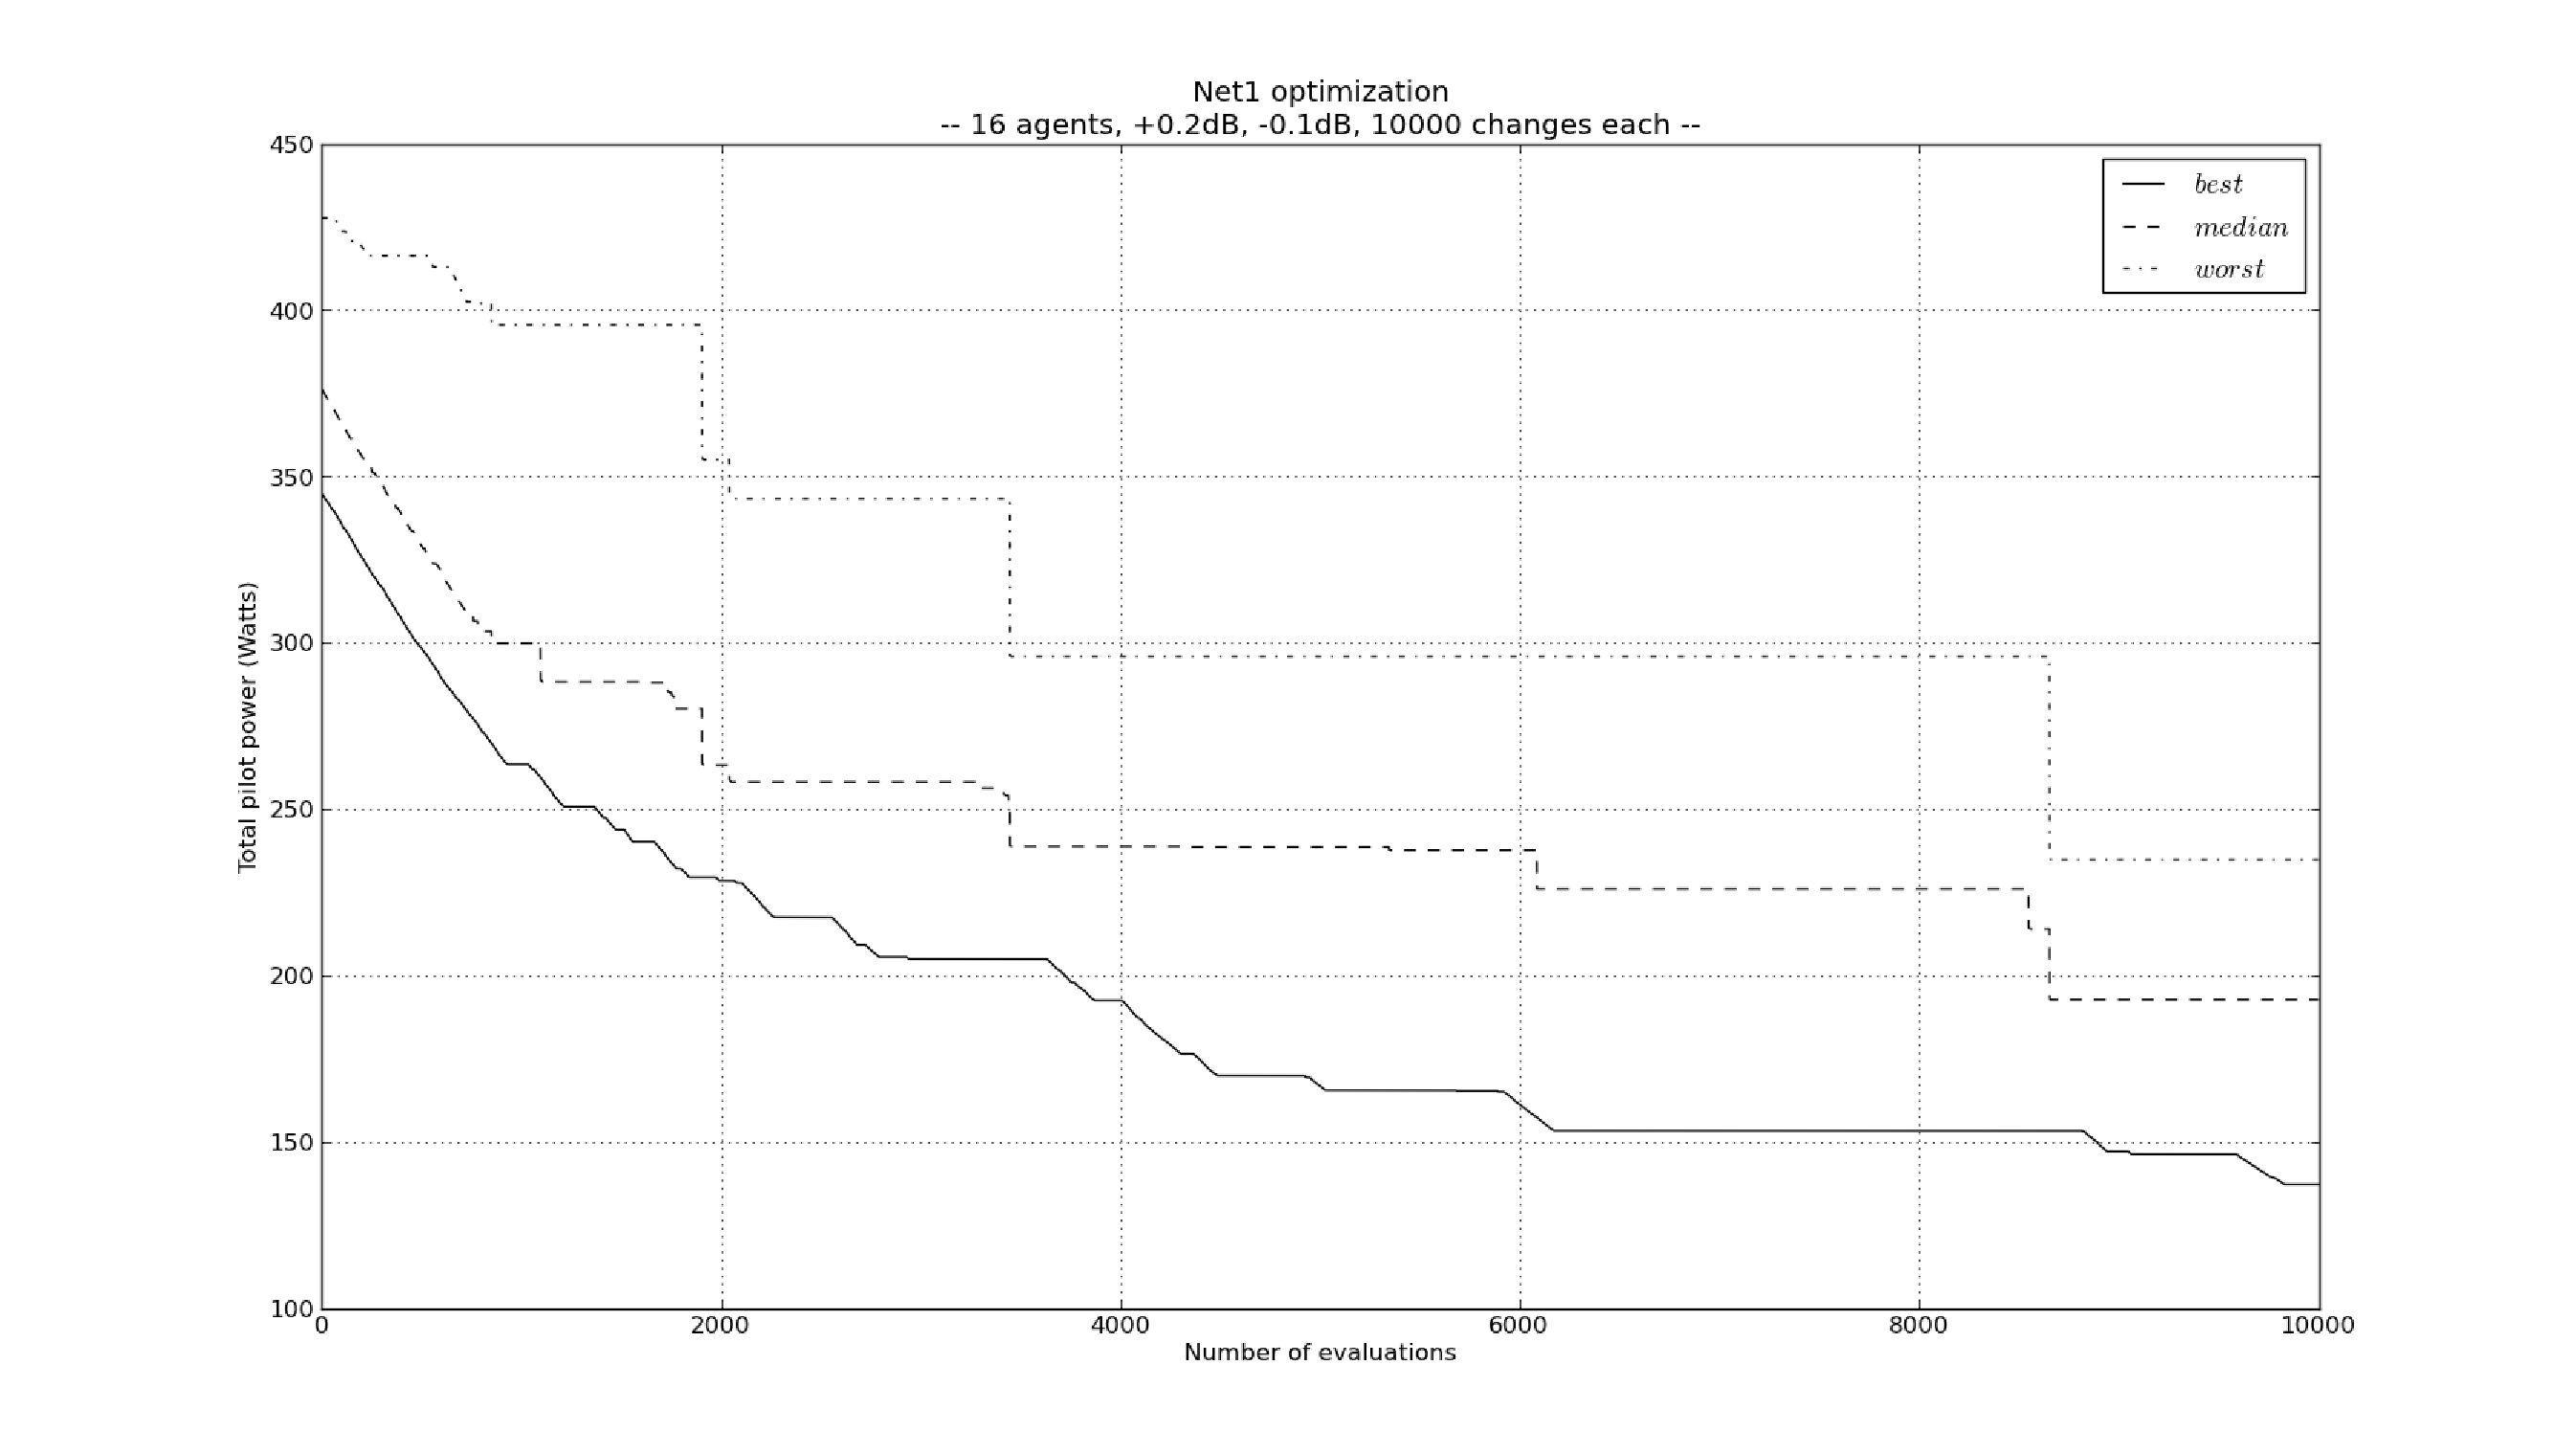
\includegraphics[width=1\textwidth]{06-experimental_evaluation-service_coverage/img/convergence_1}

\caption{\textit{Convergence results for network $Net_{1}$.\label{fig:convergence_net1}}}
\end{figure}


\begin{figure}
\centering

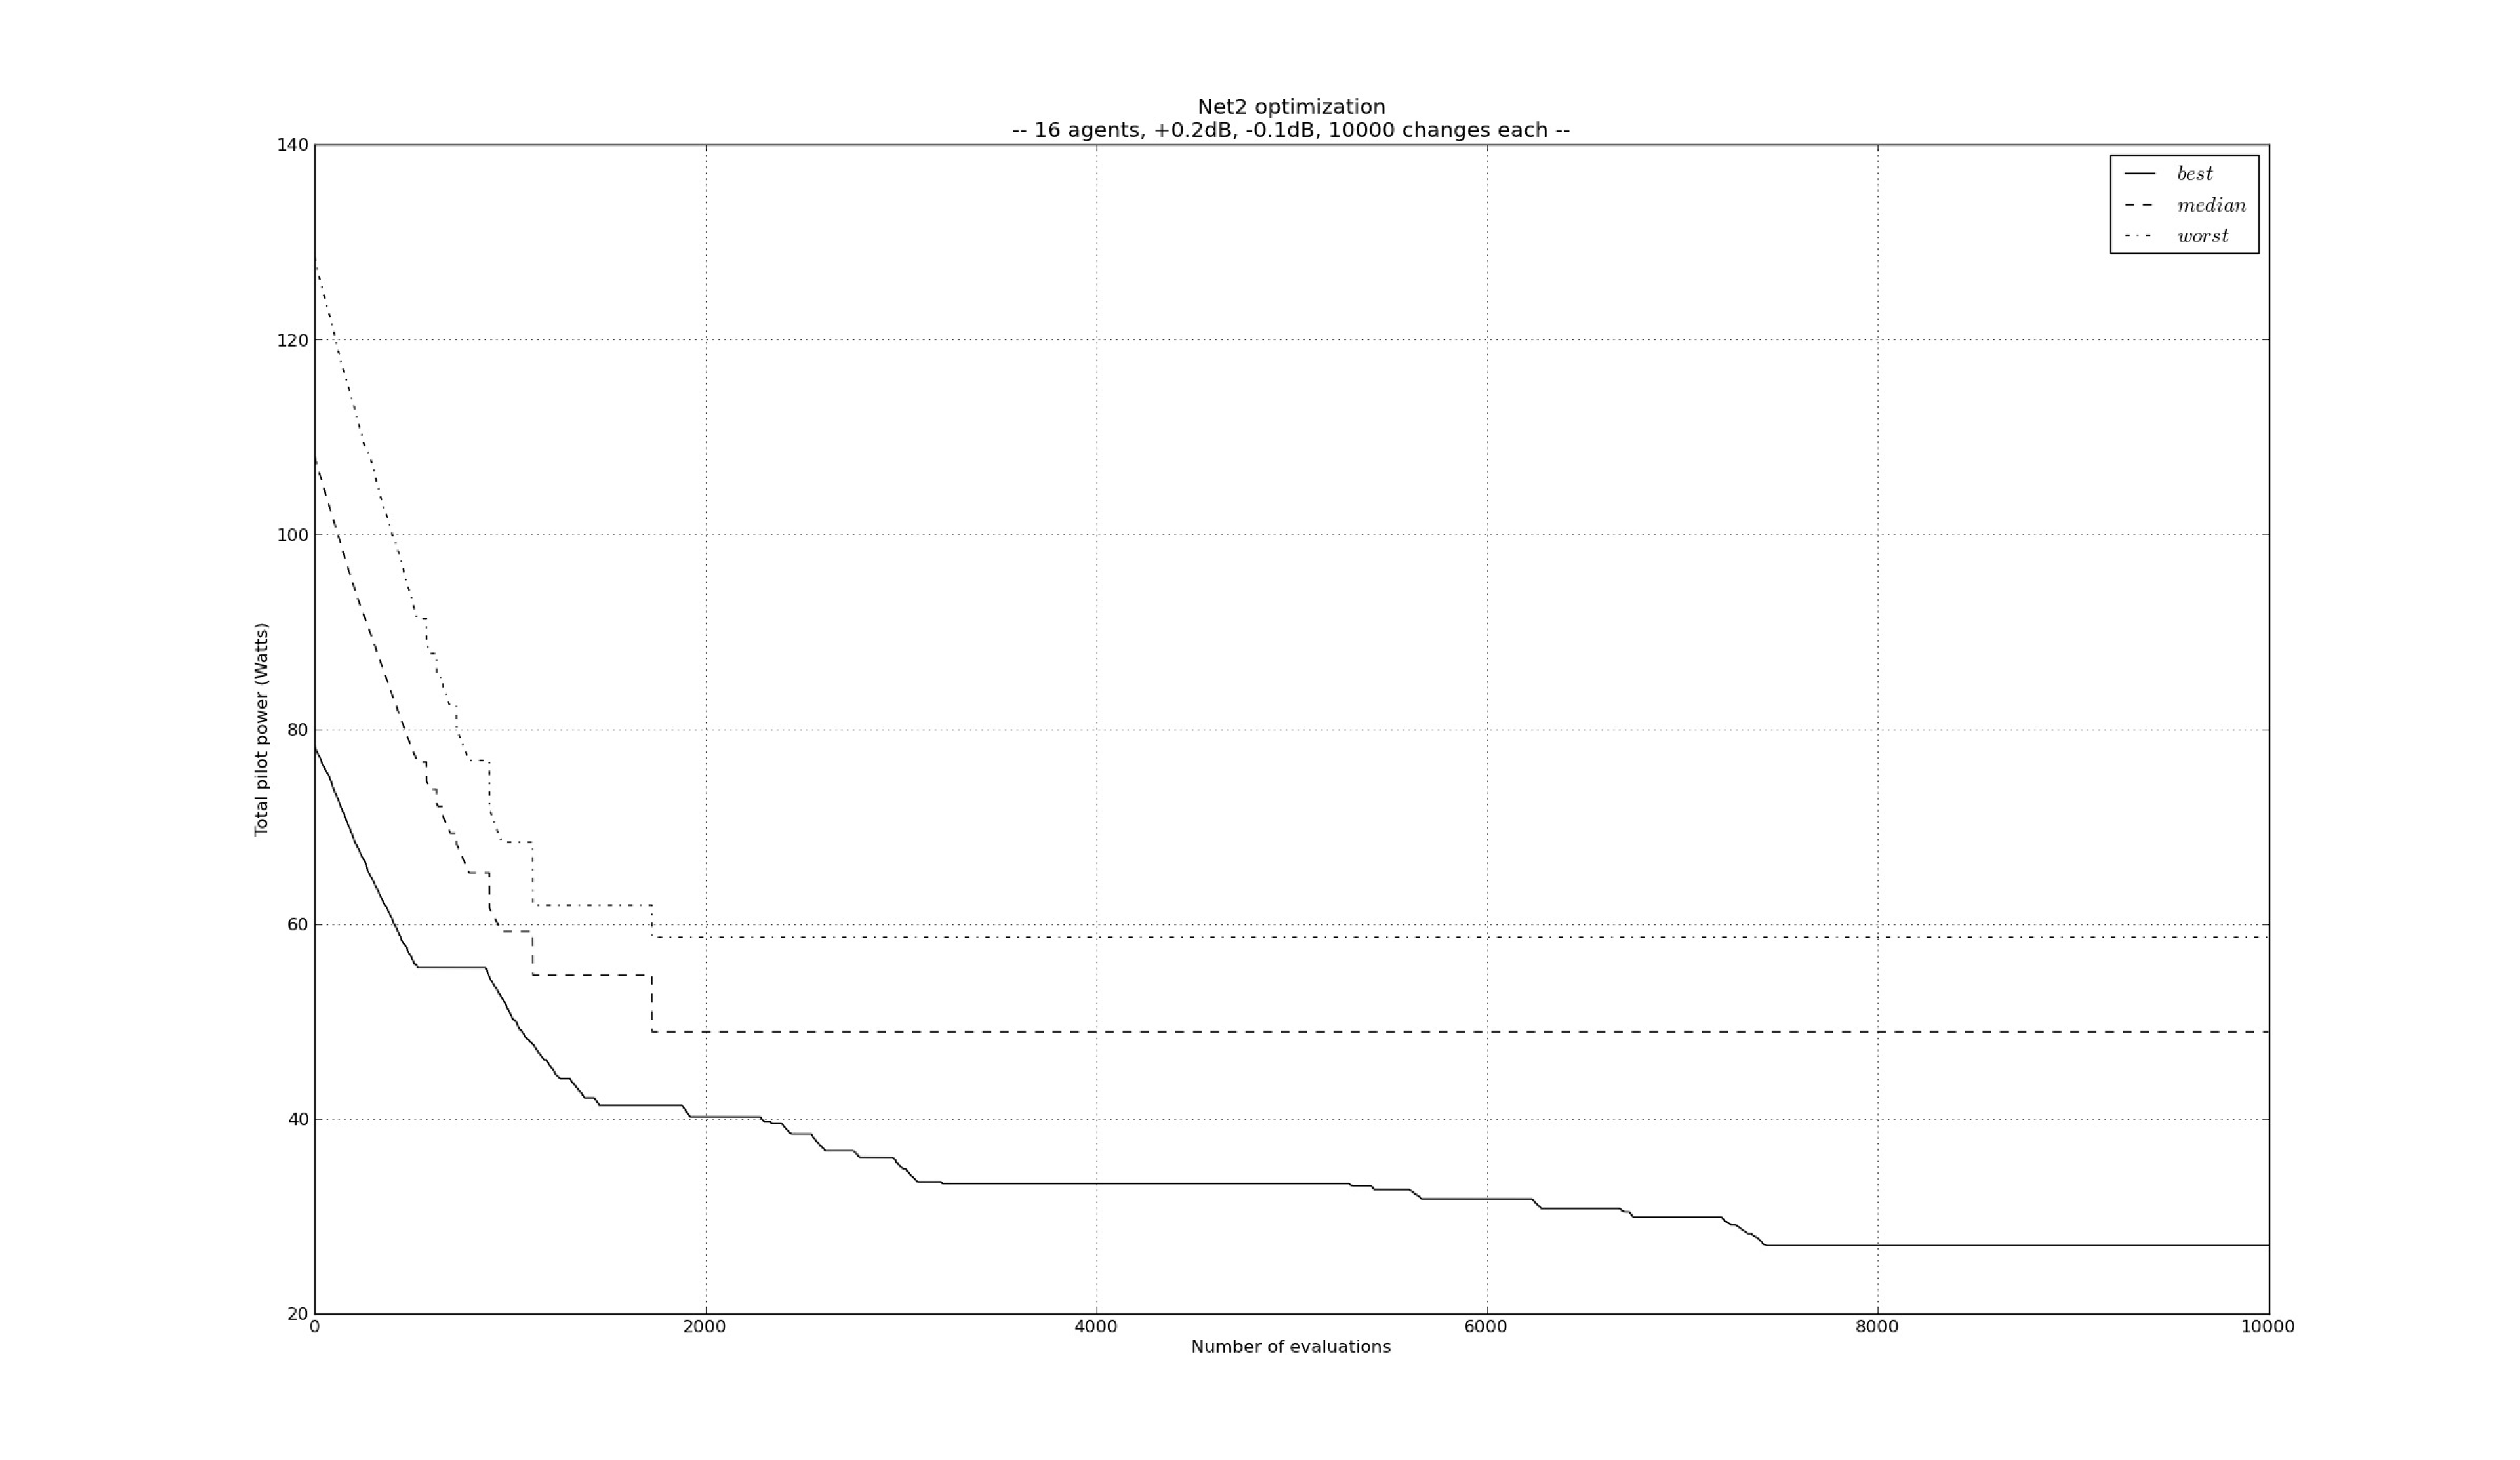
\includegraphics[width=1\textwidth]{06-experimental_evaluation-service_coverage/img/convergence_2}

\caption{\textit{Convergence results for network $Net_{2}$.\label{fig:convergence_net2}}}
\end{figure}


\begin{figure}
\centering

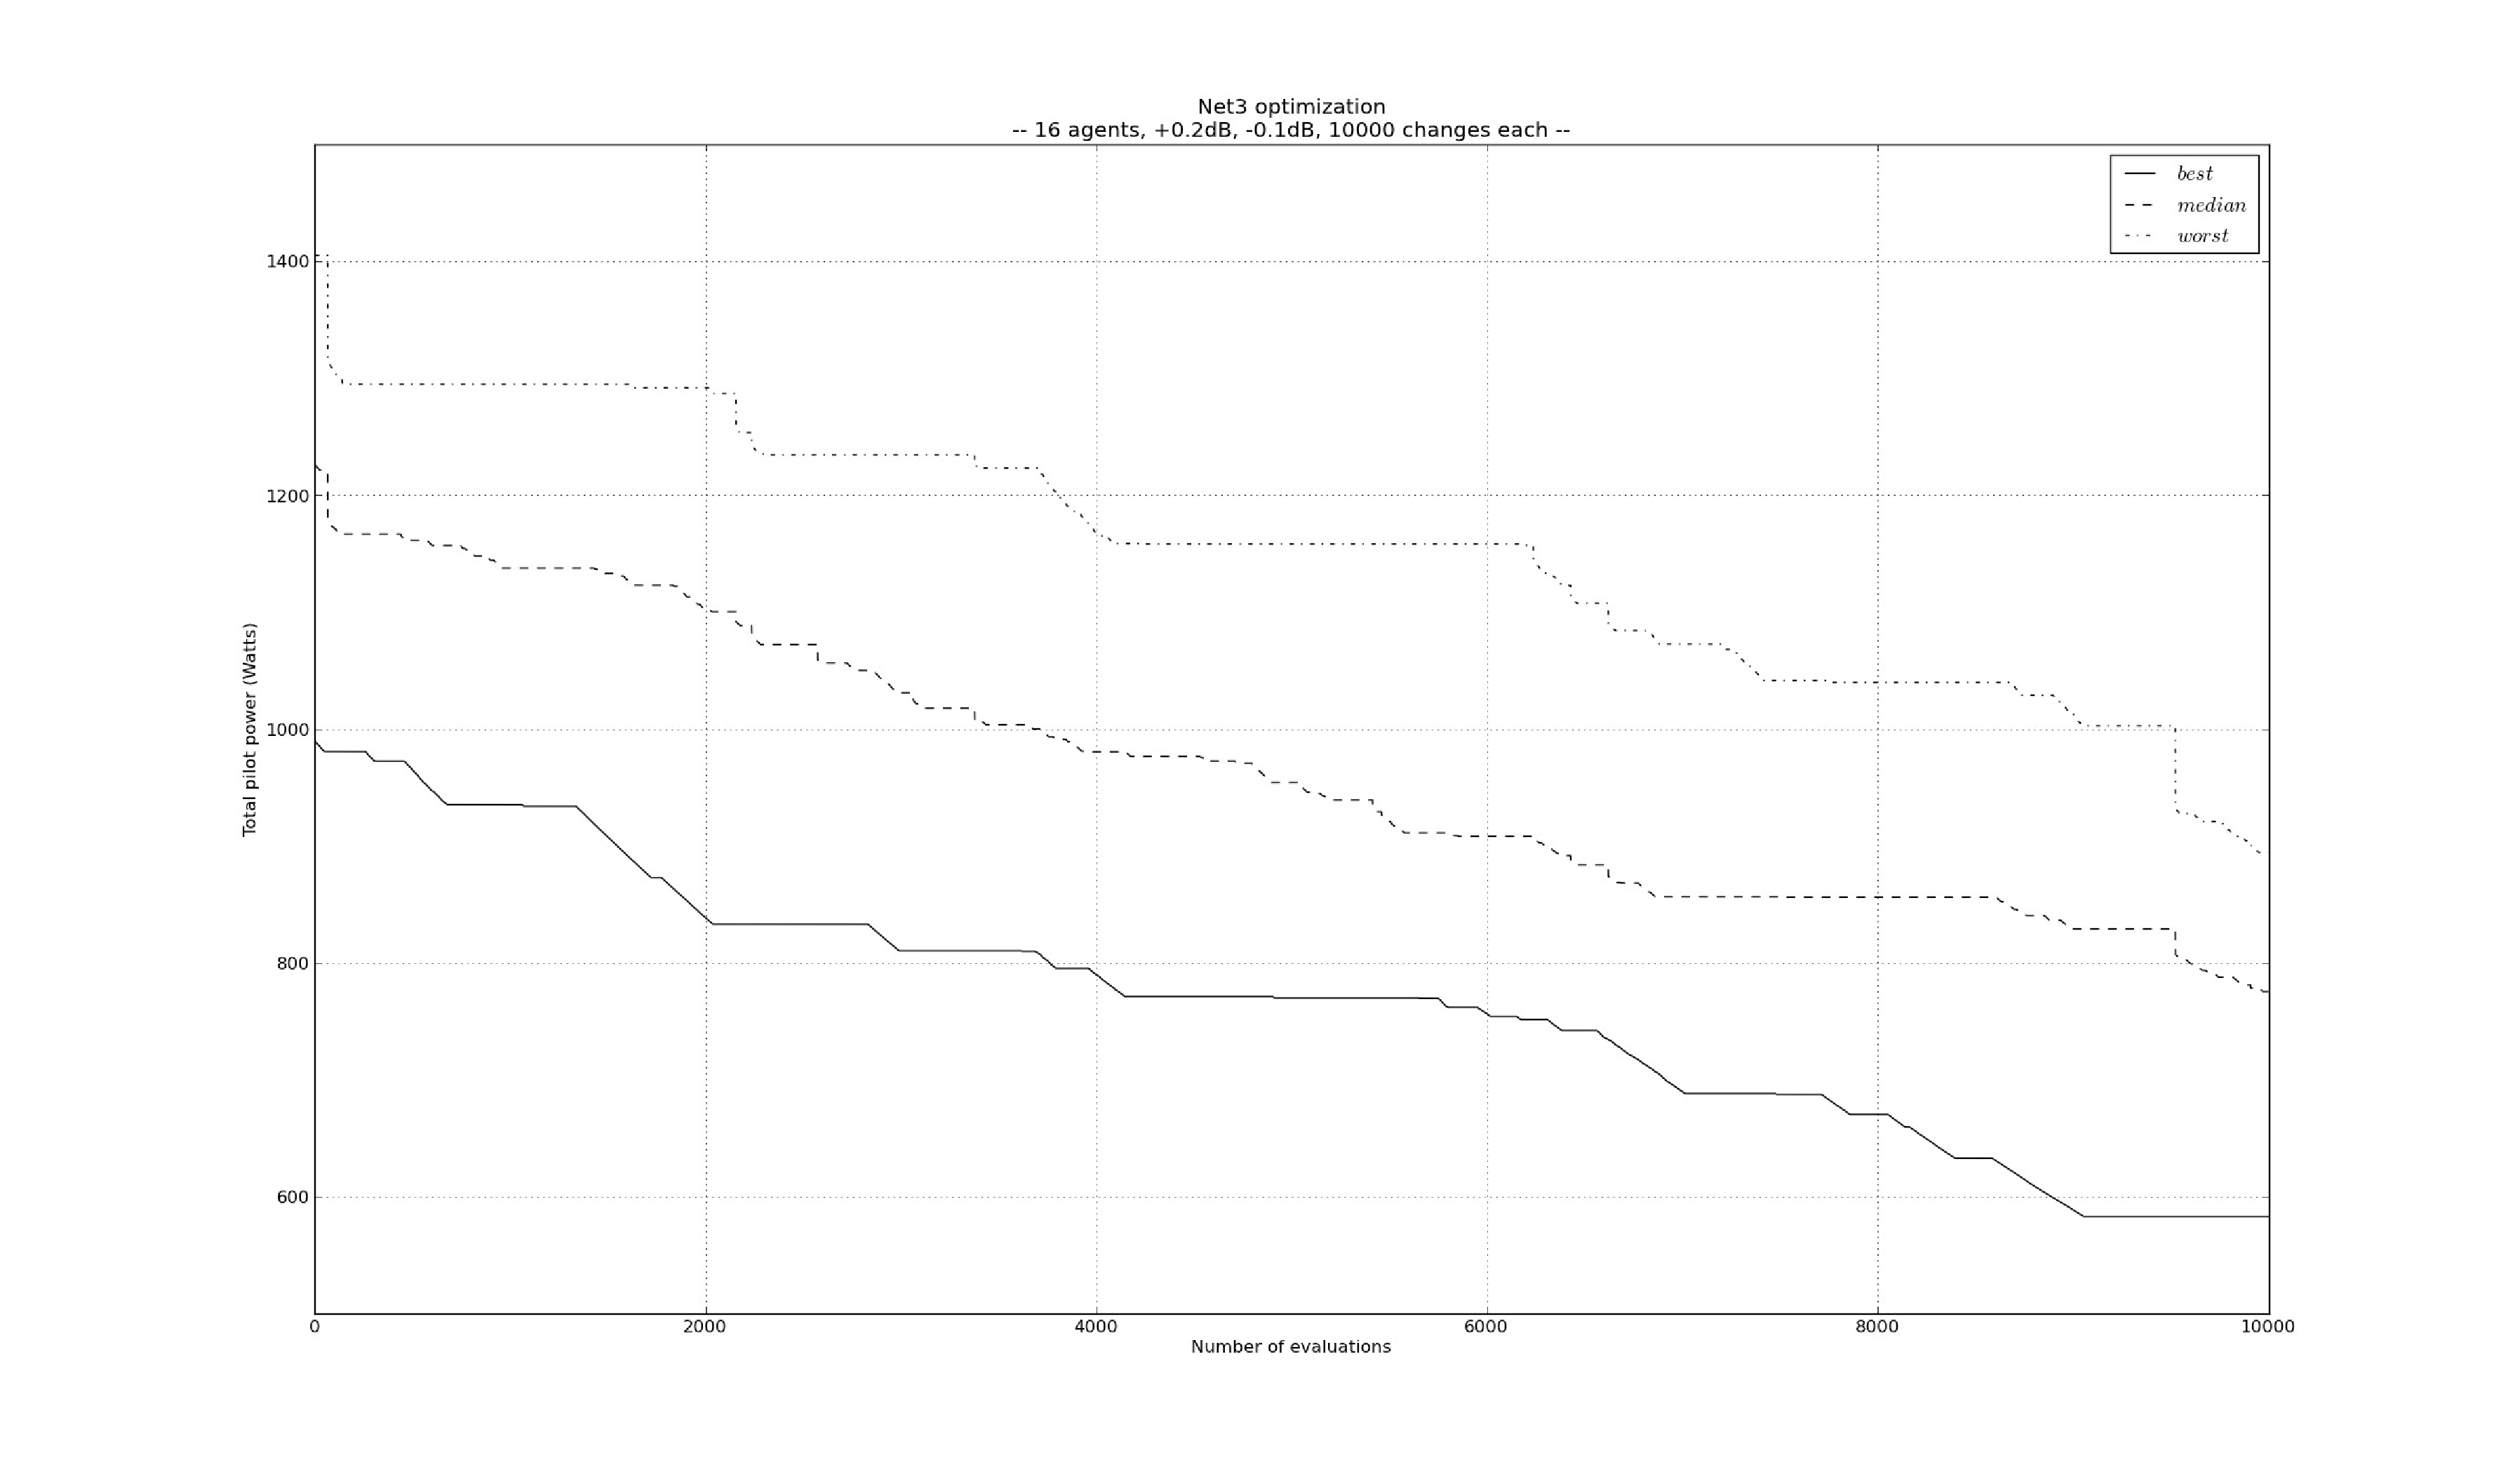
\includegraphics[width=1\textwidth]{06-experimental_evaluation-service_coverage/img/convergence_3}

\caption{\textit{Convergence results for network $Net_{3}$.\label{fig:convergence_net3}}}
\end{figure}



\subsection{Implementation results}

After measuring the quality of the solutions given by our parallel-agent
approach, we present the experimental results regarding efficiency
of different implementations. For this purpose only execution times
and speed-up factors are presented. The running time was measured
for ten independent runs on each platform. The resulting average times
are given. The number of changes per agent was limited to 100, while
all other algorithm parameters were kept at the same values as previously
stated in section \ref{sub:Algorithm-parameter-settings}.

The results, shown in Table \ref{tab:speedup-results}, are reported
for different sizes of problem instances, i.e. $Net_{1}$, $Net_{2}$
and $Net_{3}$. These networks provide different combinations of network
cells and service area size. Results are presented for a CPU-only
implementation, including objective-function evaluation on CPU and
MPI-based agents, GPU objective-function evaluation and MPI-based
agents, and GPU objective-function evaluation including agents on
the same GPU. The implementation combining CPU-based evaluator and
MPI-based agents is the basis for the speed-up calculation on the
other platforms.

\begin{table}
\caption{\textit{Implementation-efficiency measures.\label{tab:speedup-results}}}


\centering

\begin{tabular}{cccccccc}
\toprule 
 & \multicolumn{1}{c}{CPU evaluator + MPI agents} &  & \multicolumn{2}{c}{GPU evaluator + MPI agents} &  & \multicolumn{2}{c}{GPU evaluator + GPU agents}\tabularnewline\addlinespace
\cmidrule{2-2} \cmidrule{4-5} \cmidrule{7-8} 
 & Avg. time {[}sec{]} &  & Avg. time {[}sec{]} & Speed-up &  & Avg. time {[}sec{]} & Speed-up\tabularnewline\addlinespace
\cmidrule{1-2} \cmidrule{4-5} \cmidrule{7-8} 
$Net_{1}$ & 105,455 &  & 346 & 305x &  & 67 & 1574x\tabularnewline
$Net_{2}$ & 33,700 &  & 195 & 173x &  & 46 & 733x\tabularnewline
$Net_{3}$ & 191,900 &  & 506 & 379x &  & 117 & 927x\tabularnewline
\bottomrule
\end{tabular}
\end{table}


It should be noted that the MPI implementation of the agents, used
for the first and second measured setups, is not fully parallel, since
internal synchronizations at network level are performed, so agents'
changes arrive in a serial fashion to the evaluator, before being
analyzed. 

Function evaluation on the GPU communicating with agents over MPI
provides the second measured setup. The evaluator implementation takes
advantage of shared memory for thread collaboration within a block
and texture memory for constant elements, as is has been explained
in section \ref{sub:Objective-function-evaluation}. Still, the speed-up
is considerable but improvable, since numerous data transfers between
CPU and GPU are needed for the agents to access optimization-related
information.

The last result set presents measurements for complete GPU implementation,
including objective-function evaluation and agents on the same device.
The substantial speed-up delivered by this combination highlights
the great impact that CPU-to-GPU memory transfers have on overall
system performance. This fact is supported by the speed-up between
the second and third measured setups, which exhibit, on average, an
improvement of more than 400\%.


\section{Summary}

In this paper, we have addressed the problem of providing full coverage
to a service area of a UMTS network by using a minimum amount of pilot
power. We have put emphasis on the confluence of a real-world problem,
with live data from a deployed mobile network, with state-of-the-art
parallel GPU hardware and implementations that, to the best of our
knowledge, has never been dealt-with before.

We have presented a parallel-agent approach, which is aimed at giving
good solutions to big problem instances in an acceptable amount of
time. The experimental results show that our approach is able to find
competitive solutions, when compared to other common radio-planning
methods \cite{Holma_WCDMA.for.UMTS:2005}. The presented results also
demonstrate that our algorithm is able to find high quality solutions
even for large networks, that contain many cells over a large service
area. This fact indicates that our approach could be successfully
applied to bigger problem instances.

GPU architectures not only allow implementation of parallel heuristics
in a natural way, they also substantially improve the performance
of the optimization process. We reported and validated the great performance
gain by experimentation on problem instances of different sizes.

After successfully implementing the objective-function evaluation
on GPU, we realized that the efficiency of this approach was limited
by the CPU-to-GPU data transfers. Nevertheless, even with such implementation,
we have already obtained substantial speed-up.

To deal with the CPU-to-GPU data transfer issue, we implemented a
fully-enabled GPU optimization system that achieved impressive speed-up.
Still, we had to consider different data representation schemes for
the problem elements, so to avoid memory limitations on the GPU device.
Comparison of our experimental results with other algorithms dealing
with the same and similar problems would be useful. However, this
task is not straightforward, since the results of several works (e.g.
\cite{Gerdenitsch_PhD:2004,Turke_Advanced.site.configuration.techniques:2005})
depend on black-box evaluations, making experimental association very
difficult, if possible at all. 

All in all, we consider that the present work provides a robust foundation
for future work on grid-based metaheuristics with expensive objective-function
evaluation.

In future work, we will consider further analysis of our parallel-agent
approach, including experimentation with different parameters, in
order to gain better understanding of the dynamics leading the metaheuristic
during the search process. Multi-GPU environments present an interesting
possibility, where evaluator(s) and worker agents are run on separate
GPU devices.
